\begin{figure}[!h]
	\begin{center}
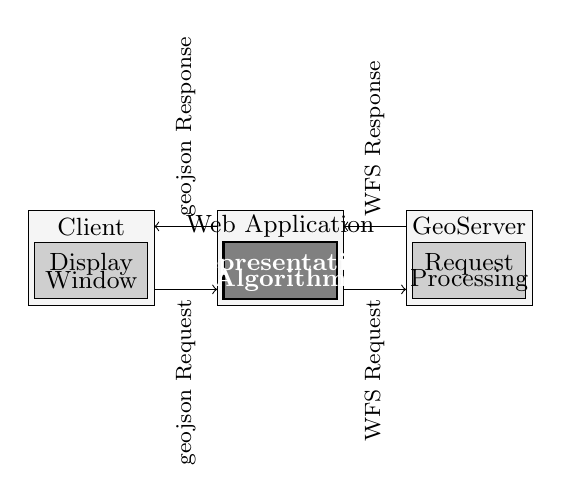
\begin{tikzpicture}[scale=0.4]
	\begin{scope}[]
		\fill[lightgray!15,draw=black] (0,0) rectangle (4,3);
		\fill[lightgray!75,draw=black] (0.2,0.2) rectangle (3.8,2);
		\node at (2,2.5) {\small Client};
		\node at (2,1.3) {\small Display};
		\node at (2,0.8) {\small Window};
	\end{scope}
	\begin{scope}[shift={(6,0)}]
		\fill[lightgray!15,draw=black] (0,0) rectangle (4,3);
		\fill[black!50,draw=black,thick] (0.2,0.2) rectangle (3.8,2);
		\node at (2,2.5) {\small Web Application};
		\node[text=white] at (2,1.3) {\small \textbf{Representation}};
		\node[text=white] at (2,0.8) {\small \textbf{Algorithm}};
	\end{scope}
	\begin{scope}[shift={(12,0)}]
		\fill[lightgray!15,draw=black] (0,0) rectangle (4,3);
		\fill[lightgray!75,draw=black] (0.2,0.2) rectangle (3.8,2);
		\node at (2,1.3) {\small Request};
		\node at (2,0.8) {\small Processing};
		\node at (2,2.5) {\small GeoServer};
	\end{scope}
	
	\begin{scope}[shift={(6,-0.5)},rotate=90]
		\draw[->] (1,2) -- node[left,rotate=90] {\footnotesize geojson Request} (1,0) ;
		\draw[<-] (3,2) -- node[right,rotate=90] {\footnotesize geojson Response} (3,0);
	\end{scope}


	\begin{scope}[shift={(12,-0.5)},rotate=90]
		\draw[->] (1,2) -- node[left,rotate=90] {\footnotesize WFS Request} (1,0) ;
		\draw[<-] (3,2) -- node[right,rotate=90] {\footnotesize WFS Response} (3,0);
	\end{scope}
\end{tikzpicture}
\end{center}
\label{fig:arch}
\end{figure}